\documentclass[lang=cn]{elegantpaper}

\title{交通灯}

\begin{document}

\maketitle

本次作业的核心是控制模块的定时转换,如果直接使用寄存器型变量,设计没有思路上的难点,但是缺乏可扩展性和整洁性,联想到上一实验中使用 \lstinline{task} 的想法,我开始探索在单个周期中使用多次 \lstinline{task} 的方式。

\section{ \lstinline{task} 初探}

本小节使用最小样例进行说明。  如 \ref{l1} 中所示,这种代码运行的结果是 \lstinline{a = b} ,而显然这是不符合我们预期的。

\begin{lstlisting}[caption={使用寄存器的任务},label={l1}]
module a(clk, a, b);
    input clk;
    output reg [3:0] a;
    output reg [3:0] b;
    reg status;
    always @(posedge clk or negedge clk) begin
        status <= ~status;
        te(a,a,clk);
        te(b,b,~clk);
    end

    task te;
    output reg [3:0] ans;
    input [3:0] data;
    input t_clk;
        begin
            ans = clk + 1;
        end
    endtask
endmodule
\end{lstlisting}

根据 IEEE-2005 标准,在 Verilog HDL 中,所有 \lstinline{task} 默认情况是静态变量,也就是单一的 \lstinline{task} 实际占据同一块内存,映射到硬件是同样的单一模块,因此实际生成的数据是在 \lstinline{b} 写入任务的数据。为了解决这个问题,只需要在 \lstinline{task} 后添加关键字 \lstinline{automatic} 就可以转换为自动的变量,在每次调用都会生成一个新的实例,解决这个问题。

\section{设计思路}

另一方面, \lstinline{task} 时序独立于调用其的模块,在执行时会阻塞调用模块的时序,据此设计可以延时任意时长的任务,如 \ref{l2} 。由于开始调用 \lstinline{task} 也会使用一个上升沿,因此所需计数需要减去一。

\begin{lstlisting}[caption={延时任务},label={l2}]
task automatic wait_and_change; 
    input [7:0] tiks;
    input [3:0] next;
    output [3:0] next_status;
    begin
        repeat (tiks - 1) @ (posedge clk);
        next_status = next;
    end
endtask
\end{lstlisting}

灯的状态采用组合逻辑完成,可以注意到,红灯是特殊的,除去本方向的其他灯亮起时,是一直亮着的。

状态转移图如 \figref{01} 。


\begin{figure}[htb]
    \centering
    \caption{转换图}\label{01}
    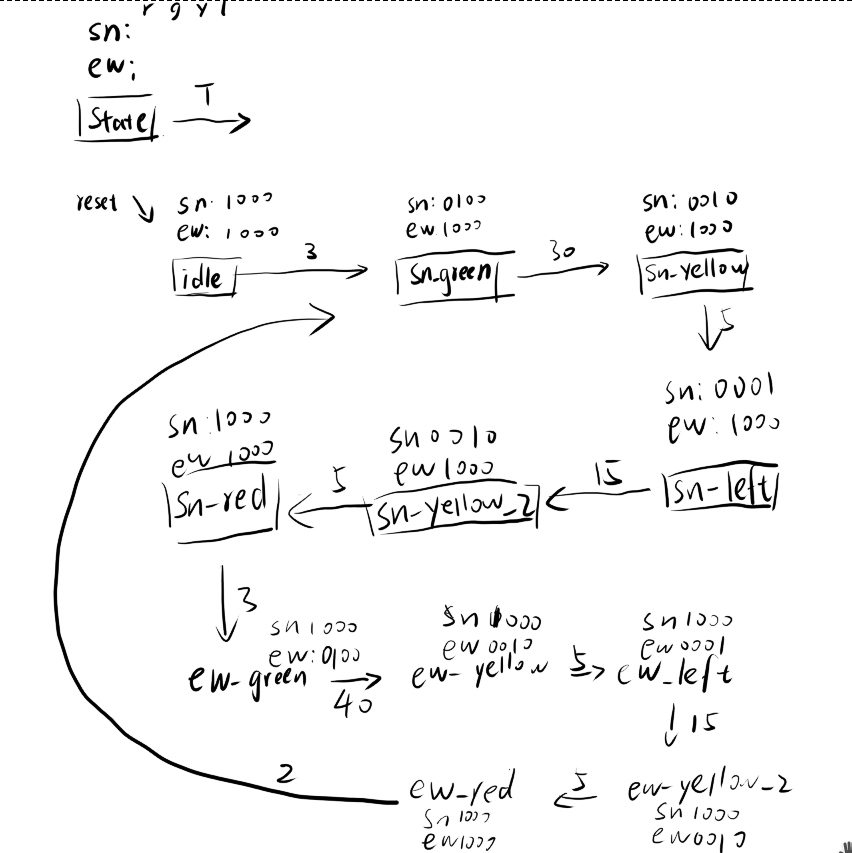
\includegraphics[width=0.6\textwidth]{fsm.png}
\end{figure}


\section{测试思路}

这道题目除了测试状态的转换,还需要测试转换持续的时间。因此,使用 \lstinline{wait} 语句检测状态是否发生可转换,并且在其中对上升沿计数,如 \ref{l3} 。

\begin{lstlisting}[caption={状态计时},label={l3}]
for (i = 0; i < 20; i = i) begin
    @(posedge clk) begin
        cnt = cnt + 1; 
    end
    if (u.status != sta) begin
        $display("state: %d, last: %d", sta, cnt); 
        sta = u.status;
        cnt = 0;
        i = i + 1;
    end
end    
\end{lstlisting}

波形序列过长,请参阅 \lstinline{test.vcd, test.wlf} 。

\end{document}
